\documentclass{jdf}

\begin{document}
Section: PUBP-6727
\title{Mutual Monitoring in the Cloud \\ Progress Report 1}
\author{Alexander Stein}

\maketitle
\thispagestyle{fancy}


\section*{Problem Statement}

Cloud computing infrastructure is essentially ubiquitous, but adoption is not without challenges. Cloud service providers must cater to customers in regulated sectors, complying with cybersecurity frameworks that create high barriers to entry. One barrier is ongoing evaluation of the provider's cybersecurity posture, often resulting in centralized bureaucracies. FedRAMP oversees and documents a prominent example of such a program, the Continuous Monitoring Program.

Are these bureaucracies an optimal solution, or a last resort that fails to keep pace with cloud technology as it proliferates and evolves? If they are a last resort, is there a better way?

\section*{Solution Statement}

I will use this research to design and evaluate an alternative to centralized continuous monitoring, mutual monitoring. The foundation of mutual monitoring will be federated data services, known in other security use cases as \hyperlink{https://transparency.dev}{transparency services}. The positives and negatives of FedRAMP's continuous monitoring model will inform its design. Operating such services should change the economics, and thereby the behavior, of cloud service providers and their customers. A new architecture should incentivize auditors to sell value-add analytics via these federated data services, potentially obsoleting centralized authorities for continuous monitoring like FedRAMP.

\section*{Completed Tasks (Last 2 Weeks)}

\begin{enumerate}
    \item I read twenty-two references (journal articles; website articles; book chapters) to identify my project in its larger context and understand supporting arguments. I concentrated on the topics below.
        \begin{itemize}
            \item primary source material from FedRAMP, especially process and procedure documentation (for  \hyperlink{https://github.com/aj-stein/practicum_proposal/blob/main/paper.pdf}{deliverable \#1})
            \item industry analysis and criticism of FedRAMP processes and their impact on FedRAMP stakeholders (for  \hyperlink{https://github.com/aj-stein/practicum_proposal/blob/main/paper.pdf}{deliverable \#1})
            \item technical methods for monitoring multi-account and multi-tenant cloud service deployments (for  \hyperlink{https://github.com/aj-stein/practicum_proposal/blob/main/paper.pdf}{deliverables \#2 and \#4})
            \item conceptual models, methods, and literature for quantitative cloud security analysis (for  \hyperlink{https://github.com/aj-stein/practicum_proposal/blob/main/paper.pdf}{deliverables \#2 and \#4})
            \item transparency service specifications (e.g. \hyperlink{https://datatracker.ietf.org/doc/draft-ietf-scitt-architecture/}{SCITT}; \hyperlink{https://c2sp.org/static-ct-api}{C2SP Static Certificate Transparency API}) and industry analysis of their efficacy (for  \hyperlink{https://github.com/aj-stein/practicum_proposal/blob/main/paper.pdf}{deliverable \#3})
            \item taxonomies and models for auditing and monitoring (for  \hyperlink{https://github.com/aj-stein/practicum_proposal/blob/main/paper.pdf}{deliverable \#2})
        \end{itemize}
    \item I presented a proposal and reviewed scope of research with four advisors that are highly familiar with FedRAMP strategy, policies, and operations. Three advisors have accepted, while one's acceptance is still pending.
    \item I began an outline for critical analysis for FedRAMP's centralized continuous monitoring model (\hyperlink{https://github.com/aj-stein/practicum_proposal/blob/main/paper.pdf}{e.g. proposal deliverable \#1}).
    \item I initialized a \hyperlink{https://github.com/aj-stein/conmotion.git}{code repository} to save the architecture documents and prototype code in version control (e.g. \hyperlink{https://github.com/aj-stein/practicum_proposal/blob/main/paper.pdf}{proposal deliverables \#2 and \#3}, respectively).
    \item I incorporated feedback from Professor Kuerbis to add and adjust research topics and evaluation methods in my \hyperlink{https://github.com/aj-stein/practicum/blob/main/notes.pdf}{outline for the project and specific deliverables}.
\end{enumerate}

\section*{Tasks for the Next Project Report}

In the next two weeks, I will focus on the following goals. I have sorted them in order of priority.

\begin{enumerate}
    \item Complete first draft of federated data service architecture, request feedback from advisors.
    \item Implement primary component of data service, submission API for cloud service providers and external third-party auditors.
    \item Complete outline of FedRAMP critical analysis.
    \item Start draft of FedRAMP critical analysis, request feedback from advisors.
\end{enumerate}

\section*{Questions or issues I'm having}

\subsection*{Alignment with Practicum Requirements}

\begin{enumerate}
    \item My project focuses on a policy challenge in cloud security, but does not have a conventional policy recommendation like other policy track proposals. Is a policy document an explicit requirement?
\end{enumerate}

\subsection*{Project Scope}

\begin{enumerate}
    \item One of my deliverables (a critical analysis of FedRAMP's current approach) is not a prerequisite I must complete to start other deliverables, but will establish important qualitative detailed background for readers, but likely it will be too detailed for the final report. Should I include this deliverable in the final report appendix or use it as an input for a summary analysis in the final report only?
    \item One of my deliverables will be a prototype of federated data service, which will have server and client components that does statistical analysis of data. There will not be a user-friendly web interface to keep scope focused and meet the projected timeline. Is this reasonable?
    \item If I cannot complete all the code for the prototype and I must scope down the prototype, do I inventory outstanding work in the future work section of the final report? Will this negatively impact my final grade for this project. Is this normal and expected?
\end{enumerate}

\subsection*{Evaluation and Measurement}

\begin{enumerate}
    \item I am proposing a novel solution that is considerably different from the current state without an ``apples to apples" comparison. It is more like an ``apples to oranges" comparison. Neither official records from FedRAMP, similar organizations, or research indicate the existence of a solution like the one I propose. There is limited data to compare my design with the current state. Is there any significant risk to my project if I design my own quantitative and qualitative metrics?    
\end{enumerate}

\section*{Methodology Paragraph Summary}

For this project, I will use multiple methods to implement an alternative architecture for monitoring cloud services and modeling its potential impact. To start, I will use a quantitative and qualitative analysis of the current shortcomings and gaps for the current FedRAMP Continuous Monitoring Program. This will be the primary example of centralized continuous monitoring for I design my mutual monitoring model for comparison. For qualitative analysis, I can perform textual analysis and sentiment analysis. I will leverage academic research, industry analysis, and a new primary source: FedRAMP's web-based forums for \hyperlink{https://www.fedramp.gov/20x/working-groups/}{the 20x reform initiative and its community working groups}. In these forums, stakeholders discuss their praise and criticism of current centralized processes and plans for future ones. In addition, I will use publicly available information from FedRAMP and industry analysis to quantify the burden of the current FedRAMP Continuous Monitoring and its manual workflow. As I build a prototype based on my architecture, I will design several use cases to estimate the cost and resource efficiency to compare those costs against the estimated costs for my solution. In addition to these methods, I will use advisors familiar with FedRAMP from different stakeholder perspectives to validate information or analysis where these methods prove lacking and leave gaps.

\section*{Timeline}

\begin{xltabular}{\textwidth}{|l|X|l|}
    % \caption{Timeline for Mutual Monitoring Project} 
    % \label{tab:timeline} \\
    \hline \multicolumn{1}{|c|}{\textbf{Week \#}} & \multicolumn{1}{c|}{\textbf{Description of Task}} & \multicolumn{1}{c|}{\textbf{Status}} \\
    \endfirsthead
    \hline
    % \multicolumn{3}{c}%
    % {\tablename\ \thetable{} -- continued from previous page} \\
    % \hline \multicolumn{1}{|c|}{\textbf{Week \#}} & \multicolumn{1}{c|}{\textbf{Description of Task}} & \multicolumn{1}{c|}{\textbf{Status}} \\ \hline 
    % \endhead
    % \hline \multicolumn{3}{|r|}{{Continued on next page}} \\ \hline
    % \endfoot    
    % \hline
    % \endlastfoot
    W1 (May 12-18) & Identify references for key research topics. & Complete \\
    \hline
    W1 & Identify advisors to review FedRAMP analysis and architecture. & Complete \\
    \hline
    W2 (May 19-25) & Initialize code repository for prototype service. & Complete \\
    \hline
    W2 & Present proposal to advisors and integrate feedback; obtain commitment from advisors. & In Progress \\
    \hline
    W2 & Read FedRAMP documentation for continuous monitoring processes. & In Progress \\
    \hline
    W2 & Begin outline of FedRAMP ConMon critical analysis. & In Progress \\
    \hline
    W3 (May 26 - Jun 1) & Implement data service internals and submission API. & Pending \\
    \hline
    W3 (May 26 - Jun 1) & First draft of data service architecture specification. & Pending \\
    \hline
    W4 (June 2-8) & Implement data service internals and submission API. & Pending \\
    \hline
    W4 & Finalize architecture specification with advisors' reviews. & Pending \\
    \hline    
    W5 (June 9-15) & Implement data service client to submit to submission API instances. & Pending \\
    \hline
    W5 & Complete data service internals and submission API. & Pending \\
    \hline
    W5 & Complete FedRAMP critical analysis document. & Pending \\
    \hline
    W6 (June 16-22) & Complete data service client to submit to submission API instances. & Pending \\
    \hline
    W6 (June 16-22) & Implement continuous monitoring quantitative processing module for API. & Pending \\
    \hline
    W6 & Design MVP continuous monitoring use cases and quantitative measurements. & Pending \\
    \hline
    W7 (June 23-29) & Complete continuous monitoring quantitative processing module for API. & Pending \\
    \hline
    W7 & Implement MVP continuous monitoring use cases in API quantitative processing module. & Pending \\
    \hline    
    W8 (June 30 - July 6) & Start prototype deployment to cloud service tenants for testing. & Pending \\
    \hline
    W9 (July 7-13) & Complete prototype deployment to cloud service tenants for testing. & Pending \\
    \hline
\end{xltabular}

\section*{Evaluation}

[Include any evaluation plans and/or results by Progress Report 4. This may expand as you finalize the report.]

\section*{Report Outline}

[Include an outline of your final report by Progress Report 4. This may expand as you finalize the report.]

\nocite{*}
\bibliographystyle{apacite}
%  Relatives path work because you initialize top-level practicum repo
%  so the paths are consistent. Clone this repo and initialize the
%  submodules and it will work.
%  https://github.com/aj-stein/practicum.git
\bibliography{../references.bib}

\section*{\centering{Appendix}}

%  Relatives path work because you initialize top-level practicum repo
%  so the paths are consistent. Clone this repo and initialize the
%  submodules and it will work.
%  https://github.com/aj-stein/practicum.git
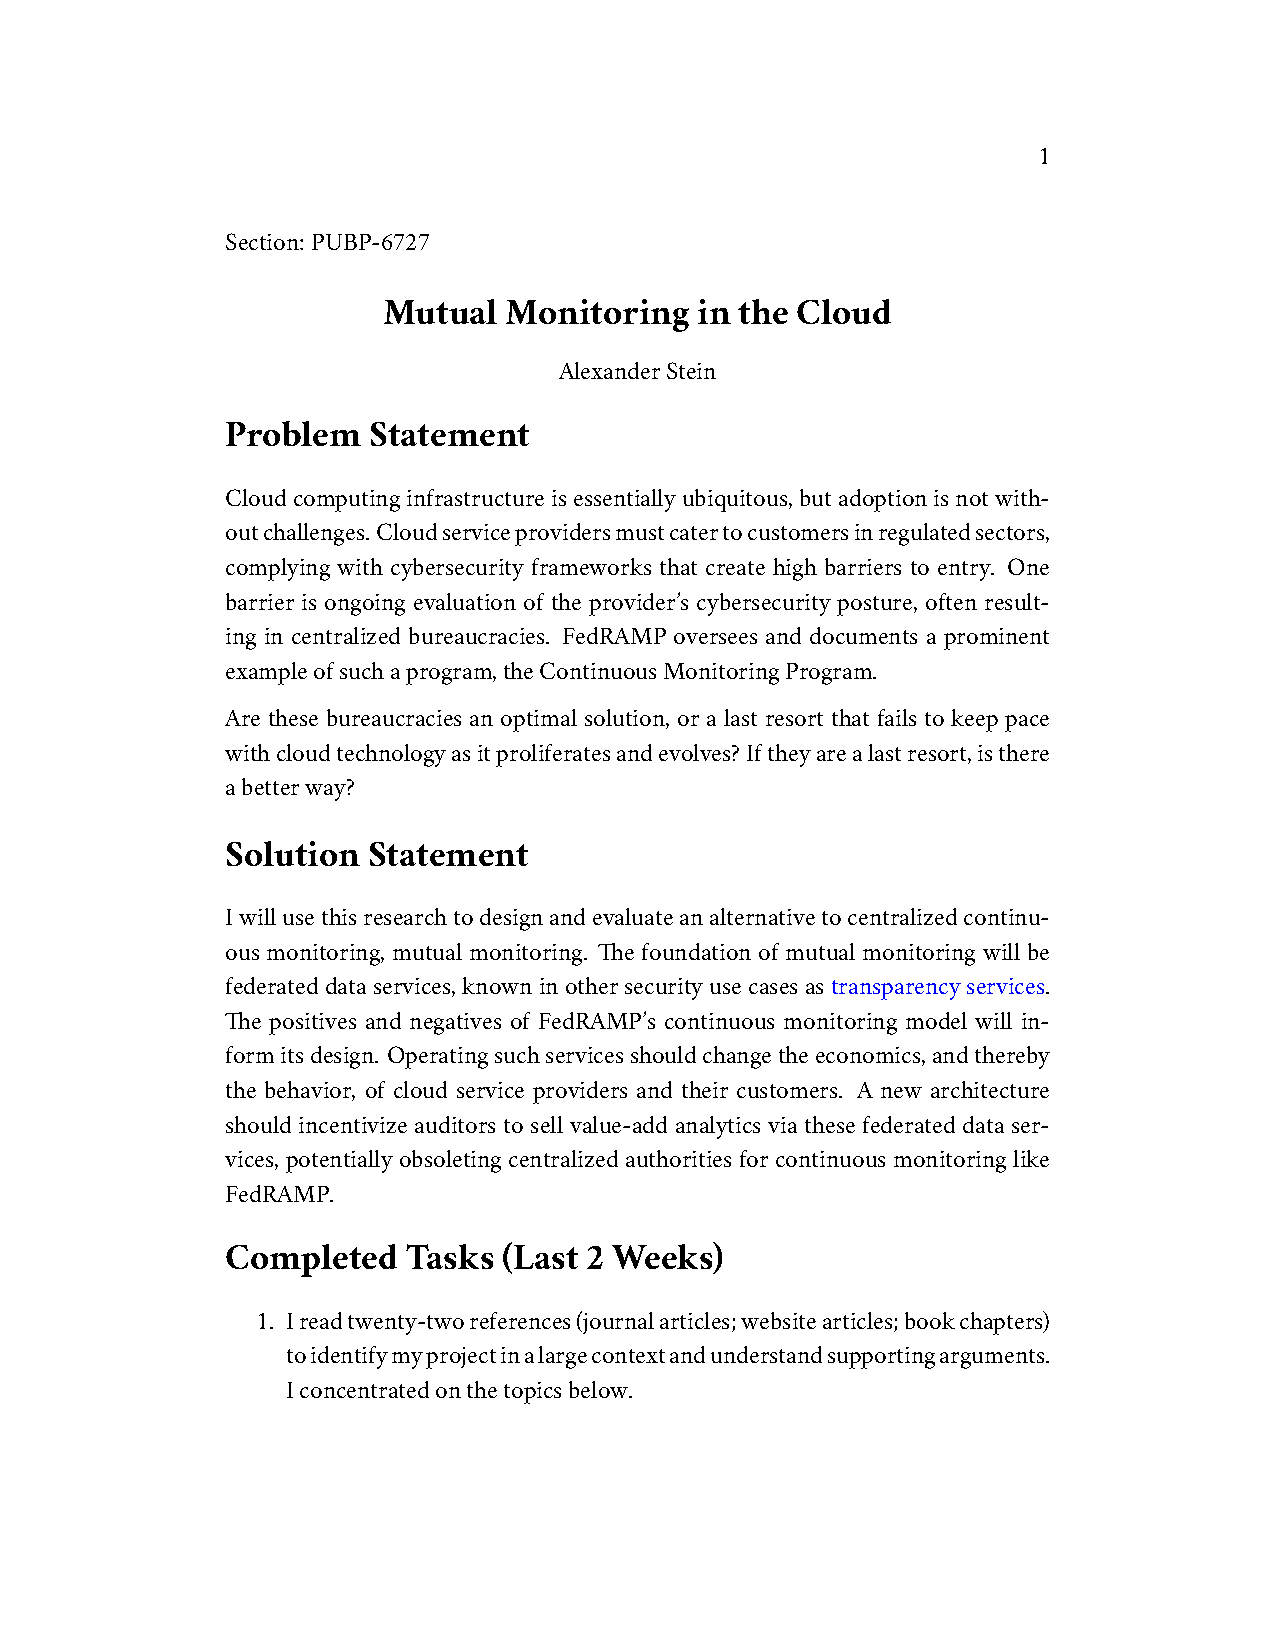
\includepdf[pages=-]{../proposal/paper.pdf}

% \subsection*{Project Outline}
% \label{appendix:outline}
% \includepdf[pages=-]{../notes.pdf}

\end{document}
